\section{Insights and Discussion}
\label{sec:discussion}
\subsection{Variable Sweeps}
\subsubsection{Hydrodynamic Efficiency}
\hl{Todo: full factorial sweep of bulk geometry variables showing maximum power and volume}
%(show MEEM sweep and power/volume pareto?)
%A full factorial sweep obtaining cw/cwmax and volume across
%m0h
%a1/a2
%m0a2
%d1/h
%d2/d1
%Nondimensionalize power by wave power and volume like I did in umerc paper

\subsubsection{Damping Plate Size}
\figureautorefname~\ref{fig:damping-plate-maxs} shows that damping plate stress can be reduced substantially by increasing the plate inner radius.
This is because the same force has a lower lever arm to the column and therefore creates less bending moment.
\begin{figure}
    \centering
    \includegraphics[width=0.75\linewidth]{\matlabFilepath{41}}
    \caption{Effect of damping plate aspect ratio on maximum stress and deflection}
    \label{fig:damping-plate-maxs}
\end{figure}

\subsubsection{Effect of PTO Force Limit}
Previous work \hl{cite} has shown that capping the PTO force can substantially reduce PTO size and cost with minimal decrease in power.
Reference \cite{mccabe_force-limited_2024} shows that for a given sea state, power decreases quadratically with decreasing force limit for the worst-case scenario of zero intrinsic reactance, and that highly reactive devices are even less sensitive to force limits.
Intuitively, the sensitivity of annual average power to force limit should be even lower when considering a range of realistic sea states, because large sea states that require higher forces are comparatively rare.
Using MDOcean, we investigate the effect of PTO force limit on average power and structural load in \figureautorefname~\ref{fig:force-power-limit}.

\begin{figure}
\centering
\includegraphics[width=.8\linewidth]{\matlabFilepath{35}}
\caption{Effect of Force and Power Limit}
\label{fig:force-power-limit}
\end{figure}

Decreasing the force limit has nearly no effect until the force limit is around 50\% of the nominal value, after which power falls off steeply.
On the other hand, after a brief region of insensitivity, the structural load for the operational design load case scales nearly linearly with the force limit.
The insensitive region exists because at high force limits, the hydrodynamic force rather than the PTO force dominates the overall load, although at force limits below a threshold, PTO load dominates.

\subsubsection{Design Space Exploration}
The OAT design sweep, shown in \figureautorefname~\ref{fig:experiments}, immediately draws attention to the float diameter $D_f$, shown with a red dashed line, as the variable with the strongest effect on the objectives.
A slight reduction in the diameter from its nominal value causes the cost to decrease close to linearly but the LCOE to skyrocket due to a substantial reduction in power generation.
Meanwhile, slightly increasing the diameter causes the power production to grow significantly but increases loads, leading to fatigue failure of the damping plate.
This is shown as blank on the diagram to indicate infeasibility.
A larger $\sim30\%$ diameter increase restores feasibility of the damping plate and achieves a roughly 15\textcent/kWh reduction in LCOE, representing the best design of the OAT sweep.
The results also point to the possibility of an even lower LCOE design with float diameter perhaps $\sim20\%$ larger than nominal, if the damping plate can be made feasible by increasing $t_d$ or $h_{1,stiff,d}$ without a major cost penalty. 

\begin{figure}
\centering
\includegraphics[width=\linewidth]{\matlabFilepath{15}}
\caption{Design of experiments}\label{fig:experiments}
\end{figure}

Besides $D_f$, the other design variable displaying a non-monotonic relationship with $LCOE$ is the force limit $F_{max}$, with an optimal at around half the nominal force limit.
Together, these insights inform the selection of the starting design for optimization, $\vec{x}_o$.
The OAT sweep also does not reveal any multimodality in the objectives, a promising sign that only a limited number of multi-starts may be necessary, although objective multimodality could still exist in other parts of the design space.
Finally, the OAT design sweep shows the highly constrained nature of the problem, with large regions of the design space infeasible.
In particular, the feasible region $1.3<D_f/D_{f,nom}<2.1$ is an ``island'' in the feasible design space, separated from the other feasible points at $D_f/D_{f,nom}<1 $ by the damping plate fatigue constraint.
Thus even without objective multimodality, multimodality exists in the Lagrangian (objective plus weighted active constraints), indicating the need for a multi-start optimization procedure as planned.

\subsection{Multidisciplinary Insights}
This section leverages the analytical multidisciplinary nature of the model to draw intuitive insights on limit cases and tradeoffs, and observe nondimensional relationships and scaling laws that would not be readily apparent in a purely numerical or single-discipline model.

\paragraph{Power Matrix Drivers}
Similar to \figureautorefname~\ref{fig:JPD-multiply} showing the multiplication of the power matrix by the JPD to obtain average power, \figureautorefname~\ref{fig:power-matrix-decomposition} further decomposes the power matrix into component matrices showing the impact of shape, drag, shape, maximum force, and PTO losses.
\hl{Describe how each matrix is found, and where there is coupling.}
\begin{figure}
\centering
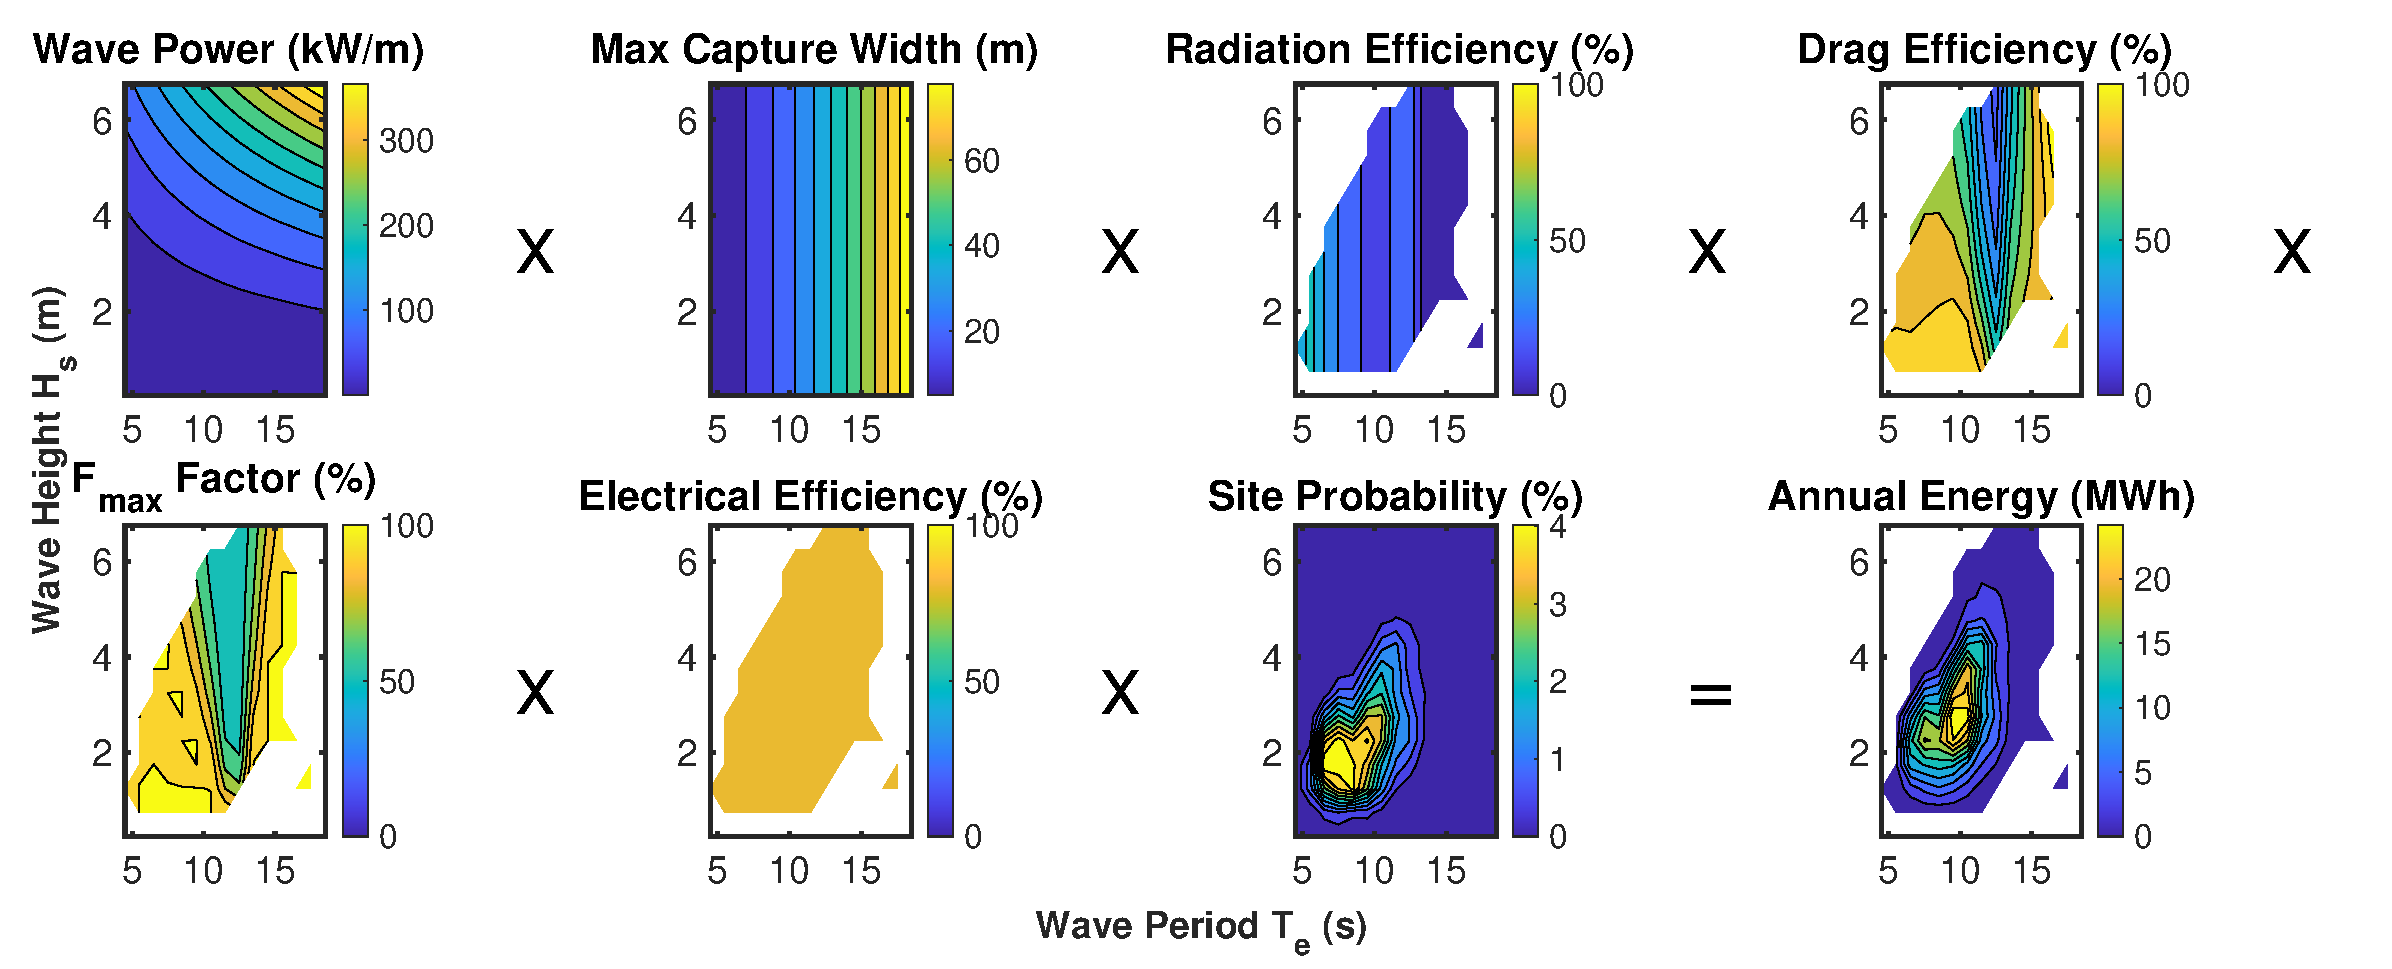
\includegraphics[width=\linewidth]{figs/power_matrix_multiply.pdf}
\caption{Power matrix decomposition}
\label{fig:power-matrix-decomposition}
\end{figure}


\paragraph{Damping vs Reactive Control}
The analytical model can be used to investigate the price conditions under which the extra power of reactive control justifies the extra cost compared to damping control.
\hl{Still in formulation, see} \appendixautorefname~\ref{sec:appendix-reactive-vs-damping}.


\subsection{Unmodeled Effects and Limitations}
\paragraph{Neglect of Surge Force}
Section~\ref{sec:dynamics} establishes that although the dynamics model estimates the surge force, the structures model uses only the heave force to calculate the factors of safety.
The neglect of surge force means that geometries with significant lateral areas that would experience high surge force perform better than they should in an optimization.
This is not only because of the impact on the structures module, but also because the surge force drives mooring cost, an effect which is not modeled in this study.
The minimum LCOE design experiences a surge force of \surgeForceFloatAtMinLCOE~on the float and \surgeForceSparAtMinLCOE~on the spar, compared to the nominal design's \surgeForceFloatNominal~and \surgeForceSparNominal~respectively.
With mooring and foundation comprising 12\% of the capital cost (see \tableautorefname~\ref{tab:CBS}), this effect may be substantial.
Incorporating surge force into the structures module and adding a mooring cost module are recommended for future work.
If these effects are implemented and confirmed to be important, then it may also be desired to obtain a more accurate estimate of the surge force across frequencies by utilizing the surge hydrodynamic coefficients instead of the long-wavelength approximation in \equationautorefname~\ref{eq:surge-force}. 

\paragraph{Regular, Linear Waves}
As section~\ref{sec:dynamics} describes, MDOcean uses standard linear wave theory with equivalent regular waves, even for the storm condition.
However, storm waves are nonlinear, and it is generally recommended to utilize higher order potential flow, CFD simulations, or wave tank tests to obtain storm loads \cite{coe_survey_2018}.
Additionally, even when storm wave analysis uses linear or quasi-linear hydrodynamics, other design procedures typically utilize a time-domain ``design wave elevation'' signal to capture transient peaks.
The regular wave analysis used in MDOcean cannot capture nonsinusoidal peaks.
Therefore, determination of design loads from a given extreme sea state represents a major area of uncertainty in this model and a challenge for future development.
Open-source tools for WEC extreme response, such as MHKiT\footnote{\url{https://mhkit-software.github.io/MHKiT/}} and the DLC Generator\footnote{\url{https://dlc.primre.org/DLCGenerator}}, apply extreme statistics to facilitate the creation of a design wave elevation but do not calculate loads from this elevation.
Finding a modeling methodology that captures hydrodynamic nonlinearities and transient peaks without optimization-prohibitive computational expense remains an open problem.
Second-order MEEM can potentially address the former, but nonlinearities require solving the radiation and diffraction problems separately, and corner discontinuities present new analytical challenges \cite{cong_novel_2020,mavrakos_second-order_2009}.
Another option is a slender-body approximation for second order loads that was recently implemented in the frequency-domain quasi-linear hydrodynamics solver RAFT \cite{carmo_slender-body_2025}.
Meanwhile, to address the transient dynamics of an irregular design wave elevation, it requires more investigation to determine whether the semi-analytical dynamics model used here can be adequately extended.
Alternatives include integrating second-order hydrodynamics into pseudo-spectral methods \cite{coe_initial_2020}, or an effort to speed up time-domain models where second-order hydrodynamics have recently been integrated.\footnote{\url{https://github.com/WEC-Sim/WEC-Sim/pull/1242}}

Besides storm loads, the regular wave assumption also affects the operational power and load calculations.
In the future, the interaction of irregular waves with dynamic constraints could be roughly approximated in MDOcean with minimal implementation effort by computing the probability density function for each signal and saturating any amplitude above the constraint threshold.
To more fully capture nonlinearities in irregular waves, the describing function mentioned earlier (which quantifies the fundamental amplitude of the response to a deterministic sinusoidal input) could be replaced with its probabilistic counterpart, stochastic linearization (which quantifies the expected value of the fundamental over the spectral input).
This technique has been explored in several WEC papers \cite{da_silva_statistical_2020,da_silva_stochastic_2023,kluger_synergistic_2017,folley_spectral-domain_2016,spanos_efficient_2016}, including one that performs multi-objective design optimization \cite{neshat_enhancing_2024}.

\paragraph{Power Variation and Grid Integration}
Additionally, while MDOcean accounts for the effect of the power limit on PTO cost, it does not directly model short-term power variation as would be necessary for sizing energy storage or grid connection, both of which would increase the effect of the power limit on cost.
In particular, the temporal alignment of power production with grid demand can affect the value of the produced electricity, and therefore the economic viability.
The authors are actively pursuing this extension, with an initial modeling process described in \cite{mccabe_wec_2025} and ongoing refinements in future work.
% other unmodeled effects to talk about later:
% MEEM damping plate, especially for spar added mass vs frequency
% MEEM non-flat bottoms
% DF for power limit
% Real PTO model
% structures model - adding local buckling, doing structural FEA validation, allowing for more prominent stiffeners using effective breadth


\subsection{Future Work}
Table~\ref{tab:future-work} summarizes potential future improvements to the model, distinguishing between model improvements that would enhance the accuracy or realism of studies that can be conducted with the present model and those that would unlock the ability to answer design questions that the current model cannot.

\newcommand{\modelTrustBuilders}{

	1) getting force with different nonlinear method: would make storm force more accurate, important since that is probably the least-theortically-defensible assumption of MDOcean

	2) more structures features: could use fatigue lifetime and in econ have lifetime = min(p.lifetime, fatigue lifetime) to be less conservative in structural sizing (currently uses endurance limit, which implies infinite fatigue lifetime)

    3) drag integral

    4) static friction describing function - ability to model static friction in drivetrain, and hydraulic check valves

    5) use extreme statistics to assess amplitude constraints, instead of max nonzero jpd
}

\newcommand{\modelStudyEnablers}{
	1) Multibody: would let me actually optimize the spar dimensions, which is important since I'm up against that constraint of min damping plate diameter

	2) Irregular waves: would let you have more realistic fatigue (ie Miner's rule), and assess power variability (ie with energy storage), which would let you see if variability reductions achieved via design are more preferable than variability reductions achieved via more batteries.
Would also give more complete results for PTO impedance matching bandwidth, ie are some PTO types or WEC shapes better Z($\omega$) shape matches with each other or with the sea state.

	3) model different WEC archetypes: would let you compare different WEC archetypes in a consistent way in the early concept design phase and start to address the design convergence problem.
Would require not only MEEM for the different WEC types, but also semi-analytical structural models for each one, or the decision to integrate a lightweight FEA with plate/shell element capabilities (ie pynite).

	4) Explicitly model the storm sea state contour 

	5) multi region MEEM: could not only make hydro coeffs more accurate representing the truncated cone shape, but would allow qualitatively different hydro coeff vs frequency shapes, which would unlock different 

	6) generator physics and model

    7) structures model for other materials
}

\begin{table}
\begin{tabular}{
        >{\centering\arraybackslash}p{0.3\linewidth}
        >{\centering\arraybackslash}p{0.6\linewidth}}
Enhance Trust in Existing Studies  & Unlock New Studies  \\ \hline
\modelTrustBuilders                & \modelStudyEnablers \\
    \end{tabular}
    \caption{Future model improvements - \hl{will be cleaned up}}
    \label{tab:future-work}
\end{table}

\paragraph{Generator physics model}
Building off the PTO CCD study that is easily realizable with the current model, a generator model would unlock control co-design with the generator itself, for example whether a high-torque (expensive) generator is worth it compared to a low torque generator.
The torque limit would essentially impose a constraint on the $F_{max}$ design var, the core losses introduce nonlinear damping, and impose a relation between generator torque limit and max/min generator inertia.
A simplified generator model is explored in the RM3 CCD study \cite{anderson_re-imagining_2024}, or a full generator model as in the offshore wind MDO study \cite{barter_beyond_2023}.

\paragraph{Structures model for other materials}
Extending the structures model to other types of materials would allow the comparison of novel WEC materials with traditional steel designs.
The existing relations between force and stress should still hold, but the relation between stress and factor of safety require modification for materials with different limit states.
This is of interest because steel accounts for a significant portion of device cost, and the assumption of steel construction may be holding the WEC industry back from economic viability.
For example, \cite{roberts_bringing_2021} found inflatable polyurethane coated nylon fabric to be more optimal than steel, reinforced concrete, fiberglass, and rubber based on basic density and cost considerations.
However, unlike ductile metals, composites require anisotropic analysis, concrete requires brittle fracture analysis such as Mohr's circle, and inflatables require tensioned membrane modeling.

\paragraph{Storm contour modeling}
Explicitly modeling the storm sea state contour as a function of location and device lifetime is possible by integrating with WDRT or a similar tool.
This is of interest in design scenarios where the WEC lifetime is a design variable.
This may prove useful to explore the tradeoffs of single-use (set-and-forget) WECs for far-offshore sensing applications where maintenance is particularly difficult or costly.